\section{תוצאות ואתגרים}

\subsection{תוצאות המודלים}
בשלב הסופי של הפרויקט נבחנה המערכת על נתוני עונת הגידול 2025, בטווח החודשים מאי--ספטמבר. המערכת כוללת שני רכיבים מרכזיים: מודל מיקרו-אקלים, המשמש להערכת תנאי הסביבה בתוך החממה, ומודל בית שורשים, החוזה את ערכי ה-pH וה-EC על בסיס מדידה נוכחית, תנאי סביבה, השקיה, דישון ומצב הצמח.

\subsubsection*{א. מודל המיקרו-אקלים}
המודל הציג רמת דיוק גבוהה בחיזוי משתני המיקרו-אקלים המרכזיים:

\begin{itemize}
    \item \textbf{טמפרטורה פנימית:} התקבל דיוק גבוה מאוד, עם מקדם הסבר של כ-\Rtwo{}=0.97 ושגיאה ממוצעת של פחות מ-0.8 מעלות צלזיוס.
    \item \textbf{לחות יחסית:} התקבל מקדם הסבר של כ-\Rtwo{}=0.87, עם שגיאה ממוצעת של כ-2.5 אחוזי לחות.
    \item \textbf{התאדות פוטנציאלית \LR{(ET0)}:} התקבל דיוק גבוה, עם \Rtwo{} של כ-0.97 ושגיאה מוחלטת ממוצעת של כ-0.016 מ"מ.
    \item \textbf{קרינה פנימית:} הקרינה בתוך החממה חושבה ונחזתה על בסיס נתוני הקרינה החיצונית ותנאי המבנה, ומהווה משתנה מרכזי להערכת עומס האנרגיה על הצמח, קצב הדיות והצטברות מלחים במצע.
    \item \textbf{טמפרטורת קרקע:} טמפרטורת הקרקע שימשה כמשתנה משלים לתיאור סביבת בית השורשים, מכיוון שהיא משפיעה על פעילות השורשים, זמינות יסודות ההזנה וקצב התהליכים הכימיים והביולוגיים במצע.
\end{itemize}

משמעות תוצאות אלו היא שמודל המיקרו-אקלים יכול לשמש שכבת קלט אמינה למודל בית השורשים. כלומר, ניתן להשתמש בו כמעין "תחנה מטאורולוגית וירטואלית" בתוך החממה.

\begin{table}[H]
    \centering
    \begin{LTR}
    \begin{tabular}{lccc}
        \toprule
        \textbf{Target Variable} & \textbf{MAE} & \textbf{\Rtwo{}} & \textbf{RMSE} \\
        \midrule
        Internal Air Temp (\textdegree C) & 0.431 & 0.972 & 0.580 \\
        Internal RH (\%)                  & 2.72  & 0.861 & 3.56  \\
        Internal Radiation                & 22.47 & 0.966 & 43.97 \\
        ET0                               & 0.0035 & 0.973 & 0.0059 \\
        Soil Temp (\textdegree C)         & 0.857 & 0.921 & 1.19  \\
        \bottomrule
    \end{tabular}
    \end{LTR}
    \caption{\LR{Overall Micro-Climate Model Performance}}
    \label{tab:microclimate}
\end{table}

\begin{figure}[H]
    \centering
    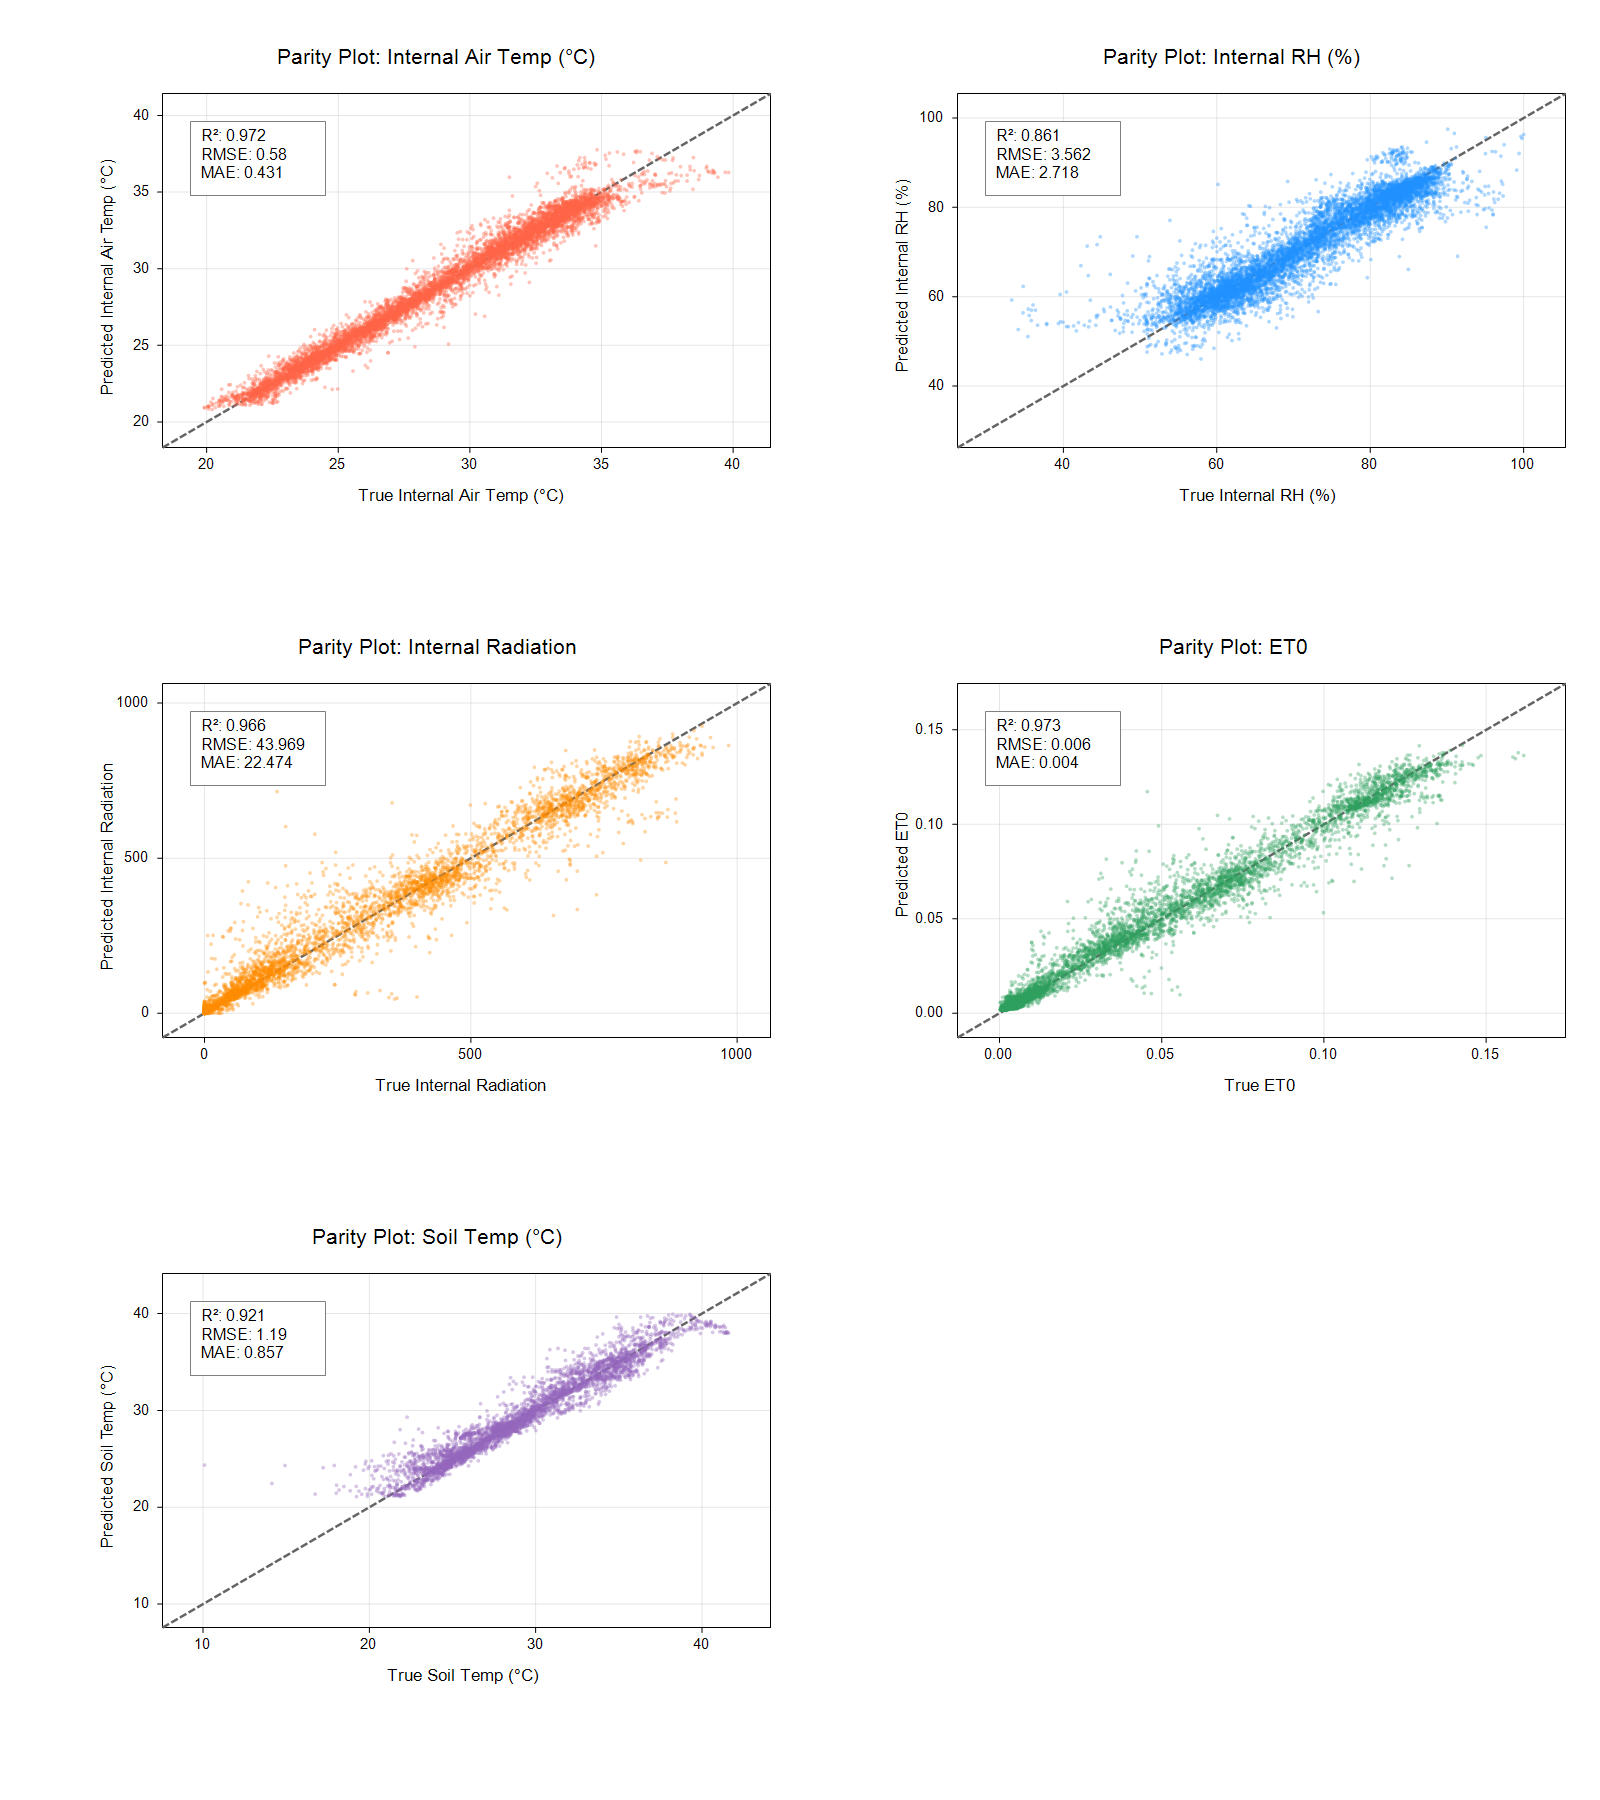
\includegraphics[width=\textwidth]{figures/fig08.png}
    \caption{\LR{Microclimate Model Results -- Parity Plot}}
    \label{fig:parity}
\end{figure}

\subsubsection*{ב. מודל בית השורשים}
מודל בית השורשים הוא מודל החיזוי המרכזי בפרויקט. המודל נבחן באמצעות \WFV{}, המדמה תרחיש שבו המודל מאומן על נתוני עבר בלבד ונדרש לחזות נקודות עתידיות. בנוסף, בוצעה בדיקת Holdout על מרווחים מדולגים, במטרה לבחון את יכולת ההכללה של המודל.

עבור pH המודל הציג ביצועים יציבים וטובים. במבחן Walk-Forward התקבלה שגיאת MAE של כ-0.33 יחידות pH, ובמבחן Holdout התקבלה שגיאת MAE של כ-0.29 יחידות pH. ערך ה-\Rtwo{} עמד על כ-0.93, והמודל שיפר את החיזוי בכ-62\% ביחס למודל נאיבי המבוסס על שמירת הערך האחרון שנמדד.

עבור EC התקבלה שגיאת MAE של כ-0.127 mS/cm במבחן Walk-Forward וכ-0.131 mS/cm במבחן Holdout. ערכי ה-\Rtwo{} היו גבוהים: כ-0.98 במבחן Walk-Forward וכ-0.95 במבחן Holdout. ביחס למודל נאיבי, התקבל שיפור של כ-35\% בדיוק החיזוי.

תוצאות אלו מצביעות על כך שהמודל מצליח ללמוד את הדינמיקה של בית השורשים מתוך שילוב של נתוני אקלים, השקיה, דישון, מצב הצמח ומדידות עבר. עם זאת, חיזוי EC נותר מאתגר יותר מחיזוי pH, בעיקר בטווחי מוליכות נמוכים שבהם גם שגיאה אבסולוטית קטנה מתורגמת לשגיאה יחסית גבוהה.

\begin{figure}[H]
    \centering
    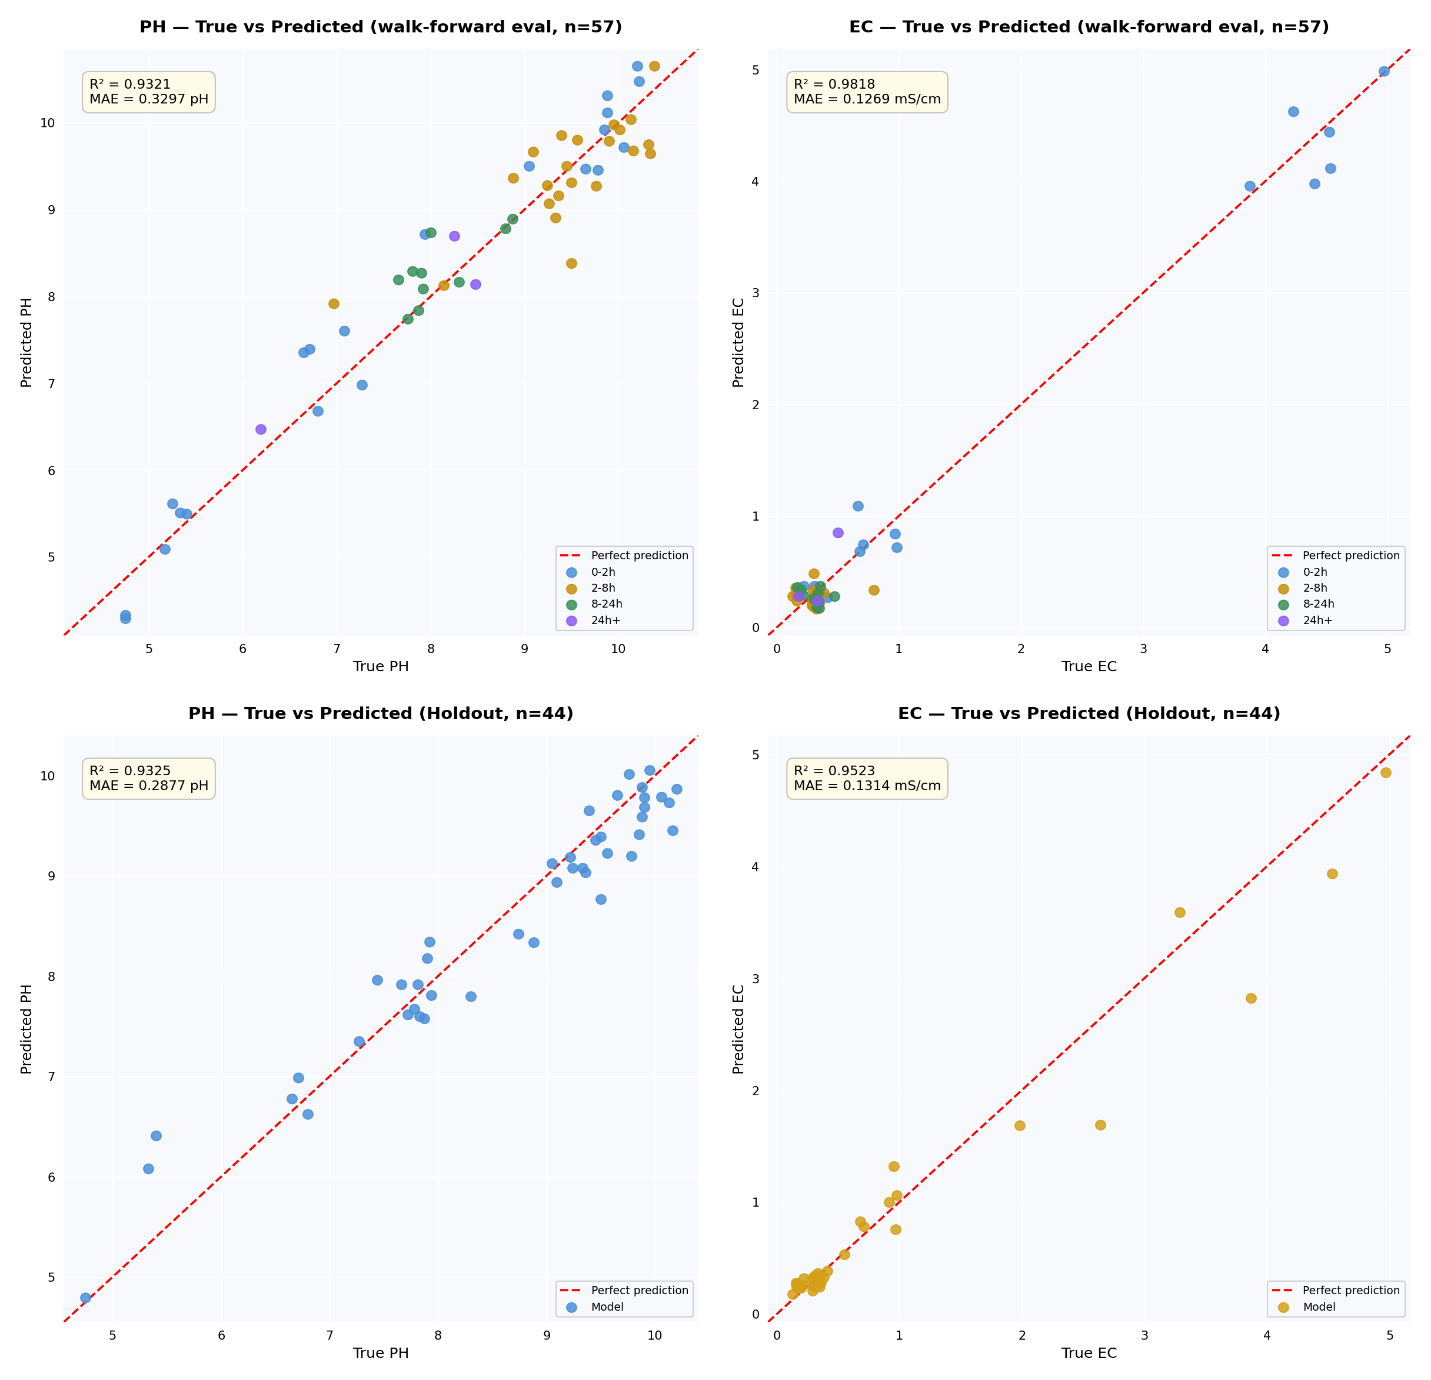
\includegraphics[width=\textwidth]{figures/fig09.png}
    \caption{\LR{Rootzone Model Results -- Scatter Plot}}
    \label{fig:scatter}
\end{figure}

\begin{table}[H]
    \centering
    \begin{LTR}
    \begin{tabular}{llccc}
        \toprule
        \textbf{Evaluation} & \textbf{Target Variable} & \textbf{MAE} & \textbf{\Rtwo{}} & \textbf{RMSE} \\
        \midrule
        Walk-Forward & pH          & 0.330 & 0.932 & 0.414 \\
        Walk-Forward & EC (mS/cm)  & 0.127 & 0.982 & 0.171 \\
        Holdout      & pH          & 0.288 & 0.933 & 0.360 \\
        Holdout      & EC (mS/cm)  & 0.131 & 0.952 & 0.255 \\
        \bottomrule
    \end{tabular}
    \end{LTR}
    \caption{\LR{Rootzone Model Performance: Walk-Forward and Holdout}}
    \label{tab:rootzone_metrics}
\end{table}

\begin{figure}[H]
    \centering
    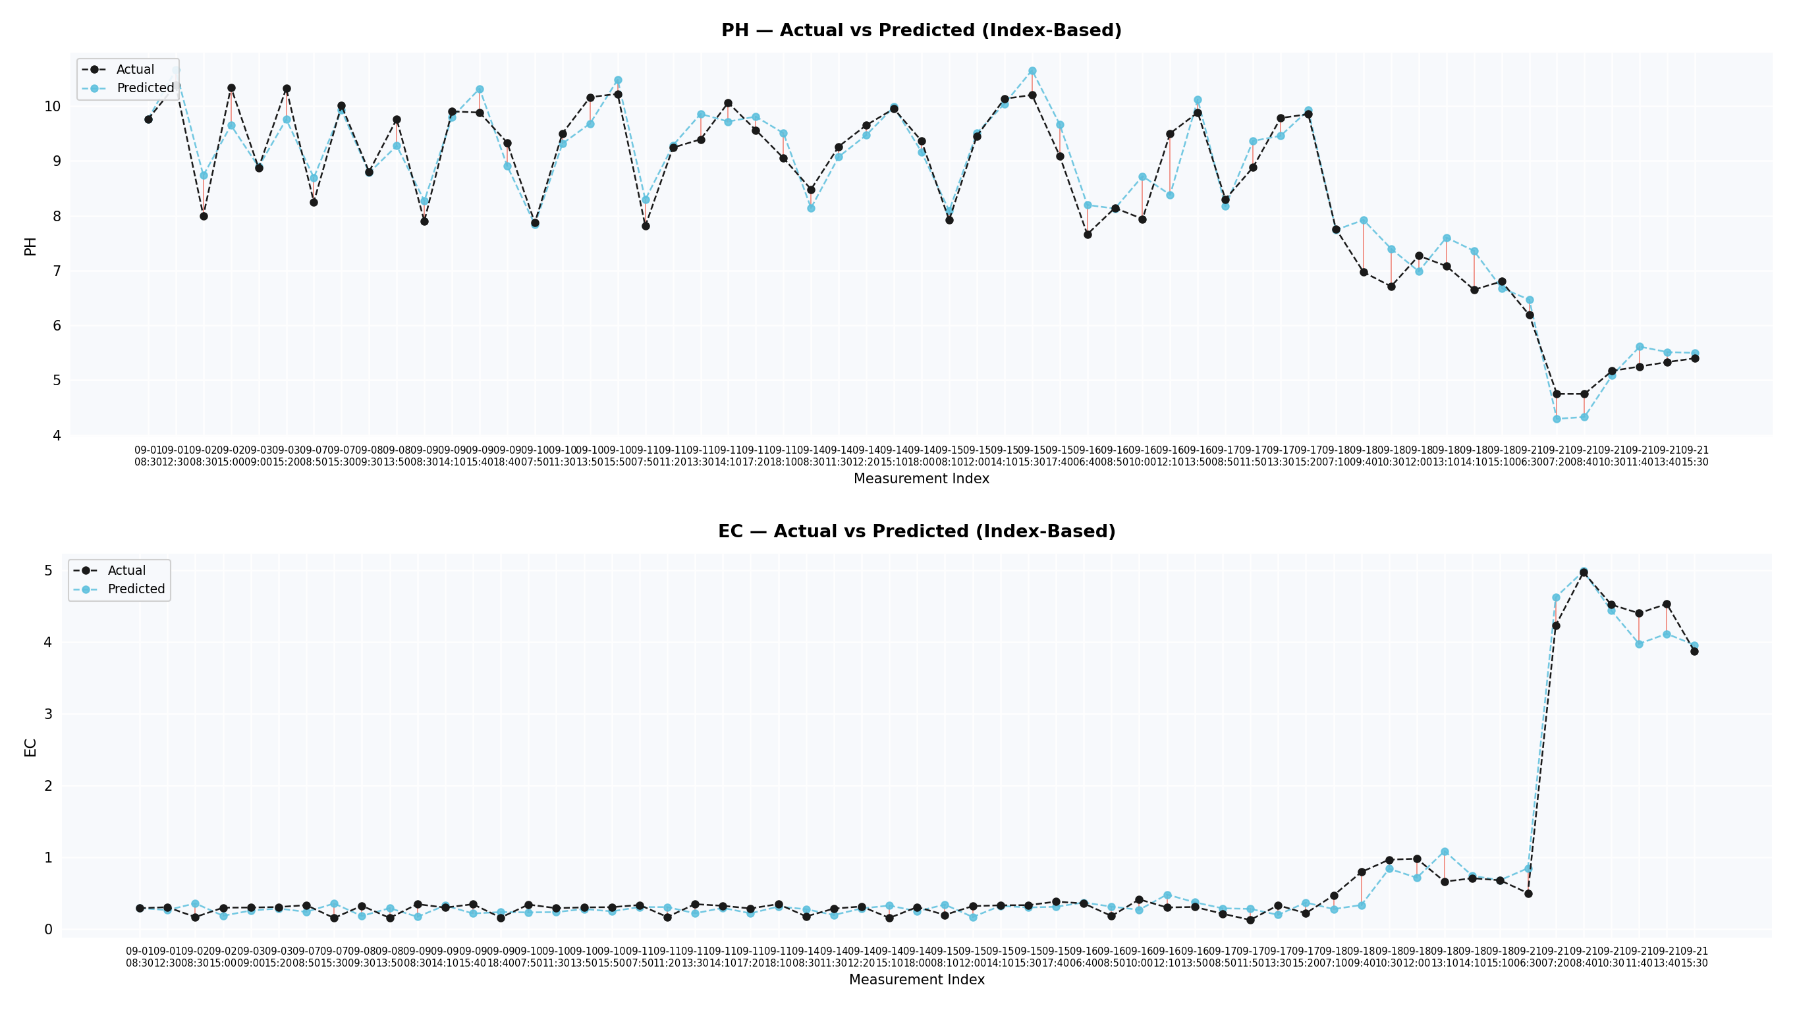
\includegraphics[width=\textwidth]{figures/fig10.png}
    \caption{\LR{Rootzone Model Results -- Time-Series Prediction}}
    \label{fig:timeseries}
\end{figure}

\begin{figure}[H]
    \centering
    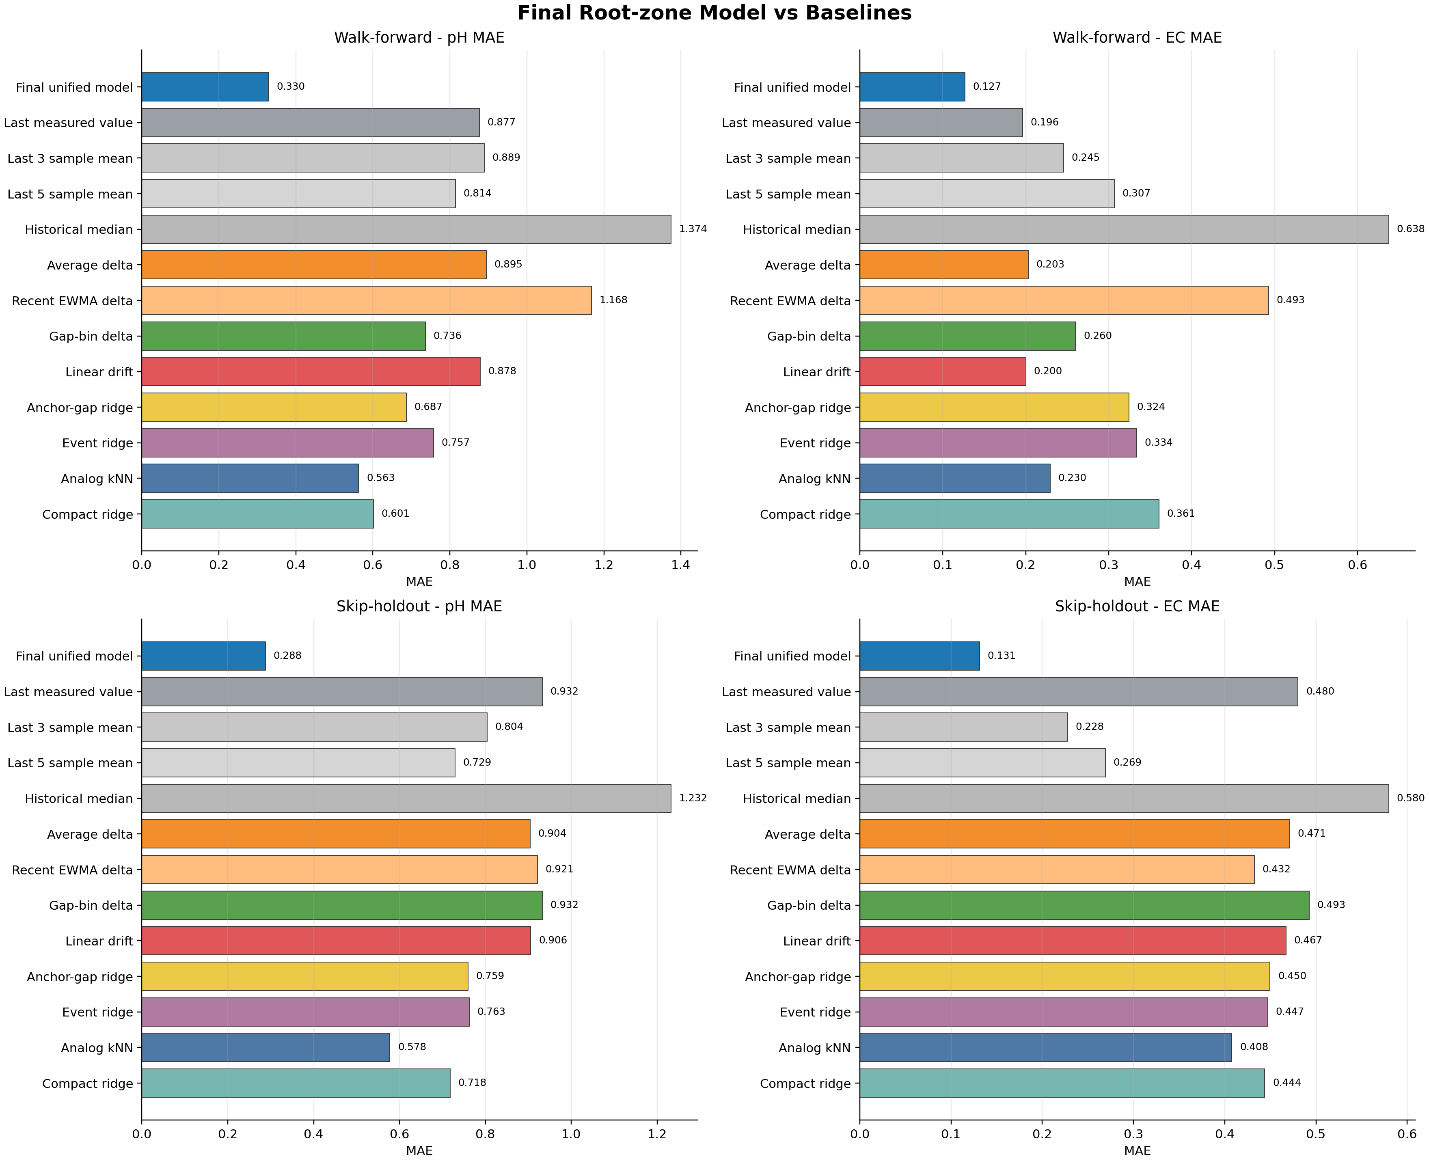
\includegraphics[width=\textwidth]{figures/fig12.png}
    \caption{\LR{Baseline Comparison -- Model vs.\ Naive Predictors}}
    \label{fig:baseline}
\end{figure}

איור \ref{fig:baseline} משווה את ביצועי המודל המאוחד הסופי מול מגוון בסיסי השוואה נאיביים (כגון שמירת הערך האחרון, ממוצע נע, וחיזוי מגמה ליניארית). בכל התרחישים -- הן ב-pH והן ב-EC, והן במבחן Walk-Forward והן במבחן Holdout -- המודל המאוחד מציג את שגיאת ה-MAE הנמוכה ביותר מבין כלל השיטות שנבחנו.

\subsection{אתגרים ודרכי פתרון}
במהלך הפיתוח נתקלנו בשישה אתגרים מרכזיים הנובעים מאופי הנתונים והמערכת. להלן הניתוח והפתרונות:

\subsubsection{"הקופסה השחורה" -- העדר ניטור רציף}
האתגר המרכזי בפרויקט הוא שבחממה הנחקרת לא הייתה מדידה רציפה של ערכי pH ו-EC בבית השורשים. ערכי האמת התקבלו מדגימות ידניות בלבד, ולכן רוב הזמן לא הייתה תמונת מצב ישירה של המצע. בין שתי דגימות ייתכנו שינויים משמעותיים במליחות או בחומציות, למשל בעקבות השקיה, דישון, אירוע חומצה, שטיפה או שינוי אקלימי, אך שינויים אלו אינם נמדדים באופן ישיר.

מצב זה יוצר "קופסה שחורה" תפעולית: ידועים לנו הקלטים למערכת, כגון מים, דשן, חומצה ותנאי סביבה, וידועות לנו נקודות מדידה בודדות של התוצאה, אך אין תיעוד רציף של התהליך שהתרחש ביניהן.

הפתרון שנבחר הוא פיתוח \SoftSensor{}, כלומר חיישן תוכנה. המודל אינו מתבסס על משוב רציף מחיישן קרקע, אלא לומד להעריך את מצב בית השורשים מתוך הנתונים הזמינים: מדידה ידועה אחרונה, תנאי אקלים ומיקרו-אקלים, השקיה, דישון, מצב הצמח והזמן שעבר עד נקודת החיזוי. בכך המודל מנסה לשחזר את הדינמיקה של המצע בין המדידות הישירות.

\subsubsection{בעיית הדלילות}
למרות שמסד הנתונים כולל אלפי רשומות אקלים ותפעול ברזולוציה של 10 דקות, מדידות היעד של pH ו-EC היו דלילות מאוד וכללו 109 נקודות מדידה בלבד. כלומר, קיימת אי-התאמה משמעותית בין כמות נתוני הקלט הצפופים לבין כמות ערכי האמת הזמינים לאימון המודל.

דלילות זו מעלה סיכון להתאמת יתר, משום שמודל מורכב עלול ללמוד רעש או תבניות מקריות במקום דפוסים כלליים. בנוסף, הדלילות מקשה על הערכת ביצועי המודל, מכיוון שכל נקודת מדידה משפיעה באופן משמעותי על המדדים הסופיים.

כדי להתמודד עם הבעיה, המודל נבנה על בסיס מרווחים בין נקודת בסיס $t_0$ לנקודת יעד $t_1$, ולא כחיזוי רציף של כל נקודת זמן. עבור כל מרווח חושבו משתני צבירה והיסטוריה המתארים את מה שהתרחש בין שתי המדידות. בנוסף, נעשה שימוש ב־\WFV{} ובבדיקת Holdout כדי לבחון את המודל בתרחיש שמדמה שימוש עתידי ולא חלוקה אקראית רגילה.

\subsubsection{רגישות המודל בערכי קיצון נמוכים}
חיזוי EC התגלה כמאתגר במיוחד בטווחי מוליכות נמוכים. בחלק ניכר מתקופת הניסוי נמדדו ערכי EC נמוכים יחסית, לעיתים סביב 0.2--0.5 mS/cm. בטווח כזה, שגיאה אבסולוטית קטנה עשויה להפוך לשגיאה יחסית גבוהה מאוד. לדוגמה, סטייה של 0.1 mS/cm היא קטנה מבחינה אבסולוטית, אך כאשר הערך האמיתי הוא 0.2 mS/cm היא מייצגת שגיאה יחסית של 50\%.

בעיה זו יוצרת קושי כפול. מצד אחד, מדדי שגיאה יחסית עלולים להחמיר יתר על המידה את הערכת המודל. מצד שני, כאשר הערכים נמוכים מאוד, יחס האות לרעש קטן: טעויות מדידה קטנות, השפעת טמפרטורה או שונות מקומית במצע עשויות להיות באותו סדר גודל כמו השינוי האמיתי בריכוז המלחים.

המשמעות האגרונומית היא שלא כל שגיאה יחסית גבוהה היא בהכרח משמעותית מבחינת קבלת החלטות. ההבדל בין EC של 0.2 ל-0.3 mS/cm עשוי להיות קטן מבחינה תפעולית, משום ששני הערכים עדיין מצביעים על מליחות נמוכה. לכן, בפרויקט הושם דגש על MAE, RMSE, \Rtwo{} והשוואה למודל נאיבי, ולא רק על אחוזי שגיאה.

כדי לשפר את יציבות החיזוי, ערכי EC עובדו באמצעות טרנספורמציה לוגריתמית של שינוי ה-EC. גישה זו מתאימה למשתני ריכוז, מפחיתה חיזויים לא פיזיקליים, ומסייעת למודל להתמודד טוב יותר עם טווחים נמוכים וגבוהים של מוליכות.

\subsubsection{אפקט הזיכרון ותלות במצב ההתחלתי}
בית השורשים אינו מגיב רק לפעולה האחרונה שבוצעה, אלא גם להיסטוריה הקודמת של המצע. לדוגמה, אותה מנת דשן עשויה לגרום לשינוי שונה לחלוטין אם היא ניתנת למצע שכבר רווי במלחים, לעומת מצע שטוף שבו ריכוז המלחים נמוך. באופן דומה, השקיה במים יכולה לגרום לדילול ולשטיפה, אך השפעתה תלויה במצב ההתחלתי, בנפח המים, בכמות הדשן ובזמן שעבר מאז אירועים קודמים.

בעיה זו מחייבת את המודל ללמוד תלות במצב. כלומר, לא מספיק לדעת מה קרה בין $t_0$ ל-$t_1$; יש צורך לדעת גם מאיזו נקודת פתיחה התחיל התהליך.

לכן הוכנסו למודל ערכי pH ו-EC בנקודת הבסיס, לצד משתני היסטוריה, משתני צבירה וחלונות זמן שונים. בנוסף, נבנו משתנים המייצגים יחסי ריכוז, כגון היחס בין כמות הדשן לבין נפח ההשקיה, כדי לייצג טוב יותר את אפקט המהילה ואת הריכוז בפועל של תמיסת ההזנה.

\subsubsection{אי-סדירות זמנית של הדגימות}
בניגוד לנתוני אקלים הנאספים כל 10 דקות, דגימות pH ו-EC לא נלקחו במרווחי זמן קבועים. לעיתים חלפו שעות בודדות בין שתי דגימות, ולעיתים יום או יותר. אי-סדירות זו מקשה על שימוש במודלים קלאסיים של סדרות עיתיות, המניחים לרוב צעד זמן קבוע.

המשמעות היא שהמודל אינו יכול להתייחס לכל מעבר בין דגימות כאילו הוא מייצג אותו פרק זמן. שינוי שהתרחש במשך שעתיים אינו שקול לשינוי שהתרחש במשך 48 שעות, גם אם בשני המקרים מדובר במעבר בין שתי מדידות עוקבות.

הפתרון היה להכניס למודל משתנה מפורש של משך הזמן בין $t_0$ ל-$t_1$, ולחשב את כלל משתני הצבירה ביחס לחלון הזמן הרלוונטי. כך המודל מקבל מידע גם על המצב ההתחלתי וגם על משך הזמן שבו הצטברו השפעות האקלים, ההשקיה והדישון.

\subsubsection{אי-רציפות בנתוני האקלים}
חלק ממדידות בית השורשים נאספו בתקופות שבהן לא היו זמינים נתוני מיקרו-אקלים פנימיים מלאים. מצב זה יצר בעיה משום שמודל בית השורשים זקוק למשתנים כגון טמפרטורה פנימית, לחות, קרינה, ET0 וטמפרטורת קרקע כדי לתאר את תנאי הסביבה שהשפיעו על הצמח והמצע.

ויתור על תקופות אלו היה מצמצם עוד יותר את מספר דגימות היעד, שגם כך היה מוגבל. לכן פותח מודל מיקרו-אקלים שלמד את הקשר בין נתוני התחנה החיצונית לבין התנאים בתוך החממה ובסביבת המצע.

באמצעות מודל זה ניתן היה להשלים או לחזות משתנים פנימיים חסרים, וליצור רצף נתונים מלא יותר עבור מודל בית השורשים. פתרון זה אפשר לנצל טוב יותר את מדידות ה-pH וה-EC הקיימות, ולשמור על עקביות בין שלב האקלים לבין שלב חיזוי בית השורשים.
